\section{Monitoring}\label{section:monitoring}

The platform contains many components and, hence, a unified logging is useful when an application is deployed. ELK Stack\footnote{\url{https://www.elastic.co/what-is/elk-stack}} is used for platform monitoring purposes. Every component can log its events over HTTP (port: 9999) or through Kafka messaging (topic: log\_collector.system\_metrics) into Logstash\footnote{\url{https://www.elastic.co/logstash}}. Only Log entities (see Appendix \ref{section:logMessage}) with defined format must be used. When a log is received by Logstash, it is stored into Elasticsearch. (The platform uses the same instance for posts, analyses, and logs.) A user can open Kibana\footnote{\url{https://www.elastic.co/kibana}} dashboard in a browser and see logs from all components in one place. Architecture is described in Diagram \ref{figure:monitoring-diagram}.

\begin{figure}[H]
\centering
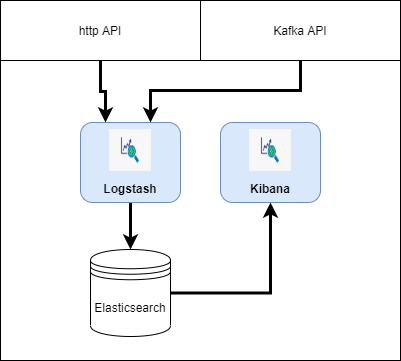
\includegraphics[width=8cm]{diagrams/socneto-metrics.png}
\caption{Diagram of monitoring interfaces. Logstash is connected to HTTP API and Kafka API and feed the data to database which is used by Kibana}
\label{figure:monitoring-diagram}
\end{figure}

\subsection{Requirements and Dependencies}

\begin{itemize}
    \item Logstash
        \begin{itemize}
            \item Minimal version of Logstash: 7.4.2
        \end{itemize}
    \item Kibana
        \begin{itemize}
            \item Recommended version of Kibana: 7.4.2
        \end{itemize}
    \item Elasticsearch
        \begin{itemize}
            \item Recommended version of Elasticsearch: 7.4.2
        \end{itemize}
    \item Kafka messaging
        \begin{itemize}
            \item Platform component
        \end{itemize}
\end{itemize}

\subsection{Configuration}

\subsubsection{Logstash Configuration}

\begin{lstlisting}[language=json,firstnumber=1]
input {
  http {
    id => "http_in"
    port => 9999
  }
  kafka {
    bootstrap_servers => "kafka:9092"
    topics => "log_collector.system_metrics"
    codec => "json"
  }
}

filter {
  if ![attributes] {
    mutate {
      remove_field => [ "attributes" ]
    }
  }
}

output {
  elasticsearch {
    hosts => [ "elasticsearch:9200" ]
  }
}
\end{lstlisting}

\subsubsection{Kibana Dashboard}

A user can specify his own dashboard with logs in Kibana. Possible fields are:
\begin{itemize}
    \item \texttt{componentId} - a name of a component
    \item \texttt{eventType} - FATAL, ERROR, WARN, INFO, METRIC
    \item \texttt{eventName} - a custom event name
    \item \texttt{message} - a custom message
    \item \texttt{timestamp} - a time when the log was created
    \item \texttt{attributes} - any JSON object with additional info
\end{itemize}